\documentclass{standalone}

\usepackage{tikz}

\begin{document}
  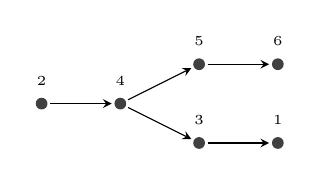
\begin{tikzpicture}
    \tikzstyle{v1} = [color=darkgray, circle, outer sep=1pt, fill, inner sep=1.5pt]
    \tikzstyle{v2} = [color=darkgray, circle, outer sep=1pt, fill, inner sep=3.0pt]
    \tikzstyle{e} = [->, >={stealth}] \tikzset{font=\tiny}

    \node[v1, label={2}] (1) at (0,0) {};
    \node[v1, label={4}] (2) at (1,0) {};
    \node[v1, label={5}] (3) at (2, 0.5) {};
    \node[v1, label={3}] (4) at (2,-0.5) {};
    \node[v1, label={6}] (5) at (3, 0.5) {};
    \node[v1, label={1}] (6) at (3,-0.5) {};
    \draw[e] (1) -- (2);
    \draw[e] (2) -- (3);
    \draw[e] (3) -- (5);
    \draw[e] (2) -- (4);
    \draw[e] (4) -- (6);
  \end{tikzpicture}
\end{document}
